\section{Aufbau und Durchführung}

\subsection{Aufbau}
\label{sec:Aufbau}

\begin{figure}[ht]
    \begin{minipage}{0.5\textwidth}
        \centering
        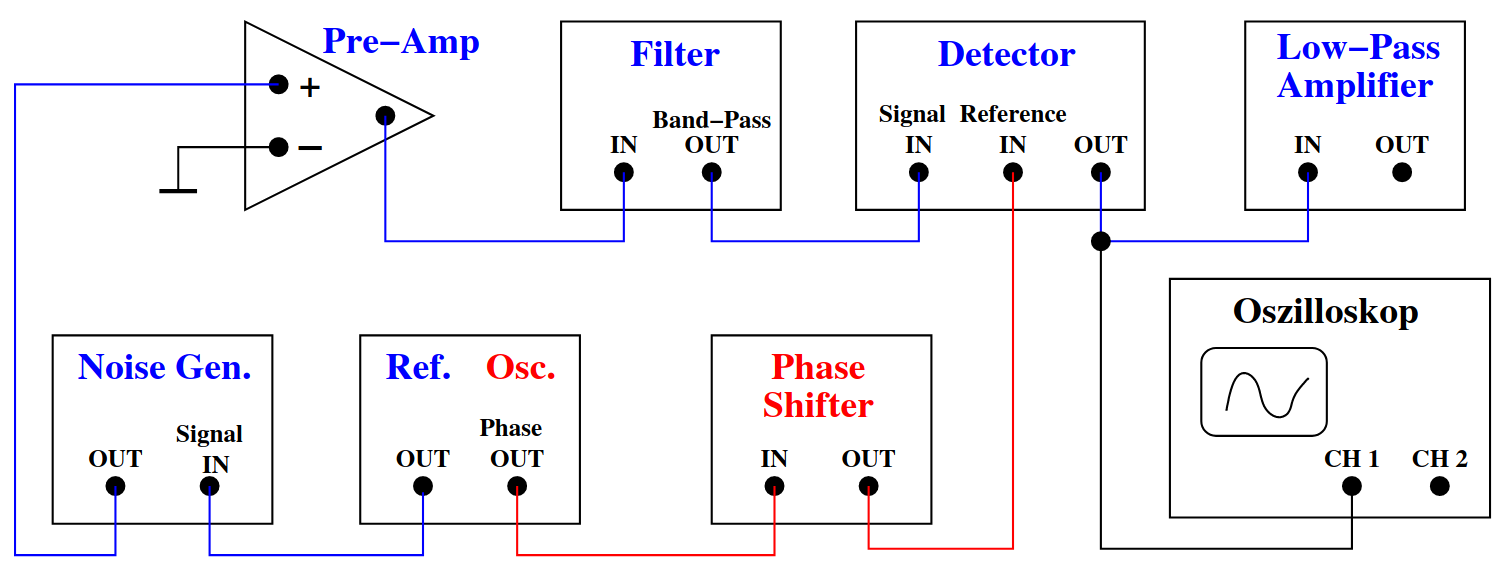
\includegraphics[width=0.4\textwidth]{img/SchematischeDarstellungLockIn.png}
        \caption{Schematische Darstellung des Lock-In-Verstärkers}
        \label{fig:SchematischeDarstellungLockIn}
    \end{minipage}
    \hspace{0.5cm}
    \begin{minipage}{0.4\textwidth}
        \centering
        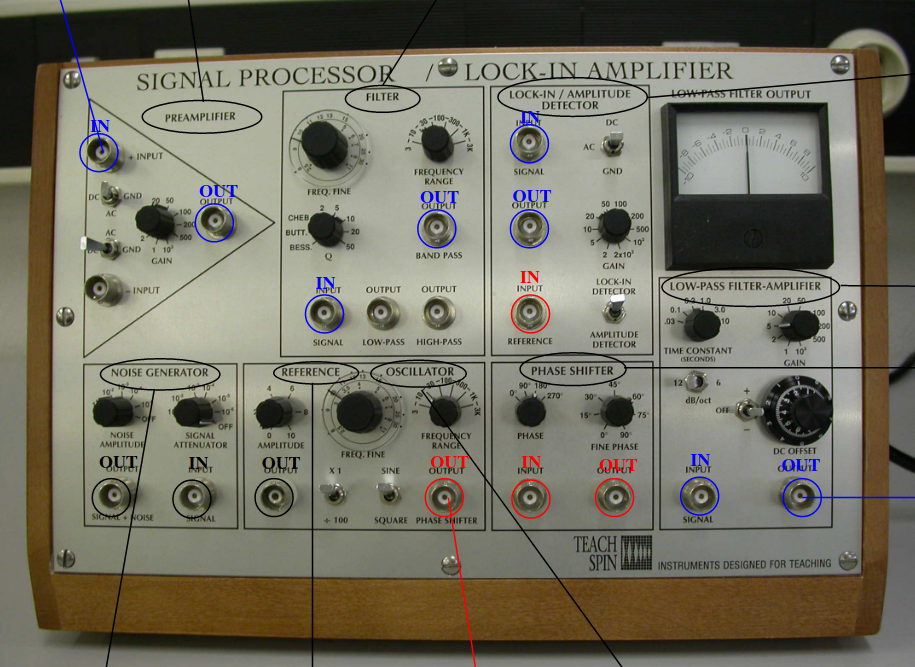
\includegraphics[width=0.4\textwidth]{img/BildLockIn.png}
        \caption{Lock-In-Verstärker}
        \label{fig:BildLockIn}
\end{figure}

Für die Versuchsdurchführung wird ein modularer Lock-In-Verstärker und ein Speicher-Oszilloskop verwendet.
Der modulare Verstärker ist in der Abbildung \ref{fig:BildLockIn} zu sehen. Es sind ein Vorverstärker, Hoch-
, Tief- und Bandpassfilter, ein Phasenschieber, ein Funktionsgenerator, ein Rauschgenerator, ein Tiefpass-Verstärker
und ein Amplituden-/ Lock-In-Detektor vorhanden. Die einzelnen Module werden per Kabel miteinander verbunden.

\subsection{Durchführung}
\label{sec:Durchführung}

Für den ersten Teil der Auswertung wird erst der Oscillator- und der Referenceoutput per Kabel an das Oszilloskop angeschlossen. 
Die relevanten Werte werden auf dem Oszillator abgelesen.\\
Für den zweiten Teil der Auswertung werden die Module wie in Abbildung \ref{fig:SchematischeDarstellungLockIn} angeschlossen.
Mit dem Oscillator-Modul wiwird ein sinusförmiges Signal $U_{sig}$ mit einer Amplitude von etwa 10 mV und einer Frequenz von 1 kHz erzeugt
und an den Verstärker weitergegeben. Der Verstärkerausgang wird mit sinus Referenzsignal $U_{ref}$ mit gleicher Frequenz gemischt.